\documentclass[12pt]{article} % Основной текст станет 12pt, а заголовки пропорционально увеличатся
%\documentclass{article}
\usepackage{graphicx} % Required for inserting images
\usepackage[russian]{babel}
\usepackage{cancel}
\usepackage{amsmath}
\usepackage{listings}
\usepackage{fancyhdr}
\usepackage{caption}
\usepackage{pdfpages}
\usepackage{amssymb}
\captionsetup[figure]{font=Large}
\DeclareMathOperator{\erf}{erf}
\usepackage{setspace} % Подключаем пакет для настройки интервала
\onehalfspacing % Устанавливаем интервал 1.5
\usepackage[
    left=30mm,      % Левое поле 30 мм
    right=15mm,     % Правое поле 15 мм
    top=20mm,       % Верхнее поле 20 мм (опционально)
    bottom=20mm,    % Нижнее поле 20 мм (опционально)
]{geometry}

\begin{document}
\Large

\section{Генерация обучающей выборки}
Для генерации обучающих данных используется два типа функций источников:

1) Гауссианы вида $f(x) = A e^{\frac{(x - \mu)^2}{\sigma^2}}$, где параметры выбираются из равномерного распределения: $A \in [1, \  10], \ \sigma^2 \in [\frac{1}{6}, \ 1], \ \mu \in [3, \ 7]$.

2) Сумма гауссиан: $f(x) = A_1 e^{\frac{(x - \mu_1)^2}{\sigma_1^2}} + A_2 e^{\frac{(x - \mu_2)^2}{\sigma_2^2}}$, параметры выбираются аналогичным образом.

Тип функции выбирается случайным образом с равным шансом. Затем выбирается $T$ из равномерного распределения на отрезке $T \in [0.1, \ 3]$. 

Всего генерируется 50000 элементов для обучающей выборки. 

\newpage
\section{Результаты расчетов}
Для каждого эксперимента выбирается $f(x), \ x > 0$ и некоторое $T$ по ним вычисляется $\varphi(x) = A_T(f)(x)$ и затем составляется обратная задача по восстановлению $f(x)$.
В каждом примере будет приведен результат работы оператора FNO и классического градиентного метода. В качестве примеров выбраны данные не из обучающей выборки, но класс функций все тот же.
Постановка задачи
\begin{align*}
        &u_t(x, t)= u_{xx}(x, t) + f(x), \ \ x  > 0, \ \ t > 0, \\
        &u_x(0, t) = 0, \ \ t > 0,\\
        &u(x, 0) = 0, \ \ x > 0,\\
        &u_t(x, T) = \varphi(x), \ \ x > 0,
\end{align*}

\newpage
\subsection{Пример 1}
$f(x) = \frac{A}{1 + \alpha(x - \beta)^2}, \ A = 5, \ \alpha = 0.5, \ \beta = 5$.
\begin{figure}[htbp]
    \centering
    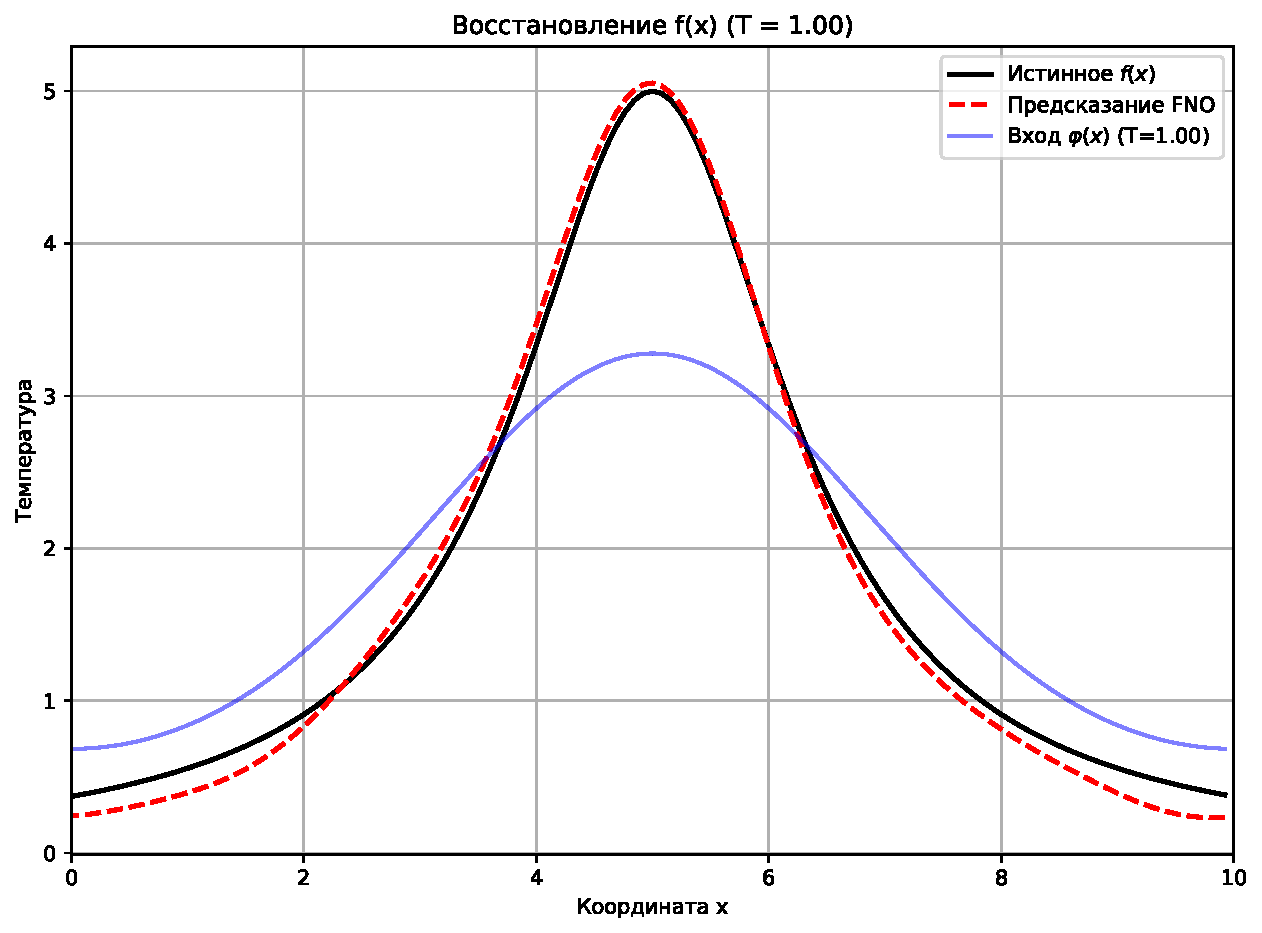
\includegraphics[width=1\textwidth]{experiment_fx0.5.pdf} 
    % width можно регулировать (например, 0.5\textwidth, или указать в см: width=10cm)
    \caption{FNO}
    \label{fig:fx1}
\end{figure}

\newpage
\subsection{Пример 2}
$f(x) = \frac{A}{1 + \alpha(x - \beta)^2}, \ A = 5, \ \alpha = 1, \ \beta = 5$.
\begin{figure}[htbp]
    \centering
    
\includegraphics[width=1\textwidth]{experiment_fx1.pdf} 
    % width можно регулировать (например, 0.5\textwidth, или указать в см: width=10cm)
    \caption{FNO}
    \label{fig:fx1}
\end{figure}


\newpage
\subsection{Пример 3}
$f(x) = \frac{A}{1 + \alpha(x - \beta)^2}, \ A = 5, \ \alpha = 2, \ \beta = 5$.
\begin{figure}[htbp]
    \centering
    
\includegraphics[width=1\textwidth]{experiment_fx2.pdf} 
    % width можно регулировать (например, 0.5\textwidth, или указать в см: width=10cm)
    \caption{FNO}
    \label{fig:fx1}
\end{figure}

\end{document}